\documentclass[12pt,twoside]{article}   
\usepackage{../../light}

\newcommand{\hint}[1]{({\it Hint: #1})}
\newcommand{\card}[1]{\left|#1\right|}
\newcommand{\union}{\cup}
\newcommand{\lgunion}{\bigcup}
\newcommand{\intersect}{\cap}
\newcommand{\lgintersect}{\bigcap}
\newcommand{\cross}{\times}

\hidesolutions
%\showsolutions

\newlength{\strutheight}
\newcommand{\prob}[1]{\mathop{\textup{Pr}} \nolimits \left( #1 \right)}
\newcommand{\prsub}[2]{\mathop{\textup{Pr}_{#1}}\nolimits\left(#2\right)}
\newcommand{\prcond}[2]{%
  \ifinner \settoheight{\strutheight}{$#1 #2$}
  \else    \settoheight{\strutheight}{$\displaystyle#1 #2$} \fi%
  \mathop{\textup{Pr}}\nolimits\left(
    #1\,\left|\protect\rule{0cm}{\strutheight}\right.\,#2
  \right)}
\newcommand{\comment}[1]{}
\newcommand{\cE}{\mathcal{E}}
\renewcommand{\setminus}{-}
\renewcommand{\complement}[1]{\overline{#1}}


\begin{document}
\problemset{11}{November 16, 2010}{Monday, November 22, 7pm}

%%%%%%%%%%%%%%%%%%%%%%%%%%%%%%%%%%%%%%%%%%%%%%%%%%%%%%%%%%%%%%%%%%%%%%%%%%%%%
%%% Fall07 ps10 problem 1

\begin{problem}{20}
You are organizing a neighborhood census and instruct your census takers
to knock on doors and note the sex of any child that answers the knock.
Assume that there are two children in a household and that girls and boys
are equally likely to be children and to open the door.

A sample space for this experiment has outcomes that are triples whose
first element is either \texttt{B} or \texttt{G} for the sex of the elder
child, likewise for the second element and the sex of the younger child,
and whose third coordinate is \texttt{E} or \texttt{Y} indicating whether
the \emph{e}lder child or \emph{y}ounger child opened the door.  For
example, $(\mathtt{B},\mathtt{G},\mathtt{Y})$ is the outcome that the elder
child is a boy, the younger child is a girl, and the girl opened the door.

\bparts

\ppart{5} Let \emph{T} be the event that the household has two girls,
and \emph{O} be the event that a girl opened the door.  List the outcomes
in \emph{T} and \emph{O}.

\solution{$T=\set{GGE,GGY}, O=\set{GGE,GGY,GBE,BGY}$}

\ppart{5} What is the probability $\prcond{T}{O}$, that both children are
girls, given that a girl opened the door?
\solution{1/2}

\ppart{10} Where is the mistake in the following argument for computing $\prcond{T}{O}$?

\begin{quote}
If a girl opens the door, then we know that there is at least one girl in
the household.  The probability that there is at least one girl is
\[
1 - \prob{\text{both children are boys}} = 1 - (1/2 \times 1/2) = 3/4.
\]
So,
\begin{eqnarray*}
\lefteqn{\prcond{T}{\text{there is at least one girl in the household}}}\\
& = & \frac{\prob{T \intersect \text{there is at least one girl in the household}}}
{\pr{\text{there is at least one girl in the household}}}\\
& = & \frac{\prob{T}}{\pr{\text{there is at least one girl in the household}}}\\
& = & (1/4) / (3/4) = 1/3.
\end{eqnarray*}
Therefore, given that a girl opened the door, the probability that there
are two girls in the household is \textup{1/3}.
\end{quote}

\solution{The argument is a correct proof that 
\[
\prcond{T}{\text{there is at least one girl in the household}} = 1/3.
\]
The problem is that the event, $H$, that the household has at least one girl,
namely,
\[
H = \set{\mathtt{GGE,GGY,GBE,GBY,BGE,BGY}},
\]
is not equal to the event, \emph{O}, that a girl opens the door.  These
two events differ:
\[
H-O = \set{\mathtt{BGE,GBY}},
\]
and their probabilities are different.  So the fallacy is in the final
conclusion where the value of $\prcond{T}{H}$ is taken to be the same as
the value $\prcond{T}{O}$.  Actually, $\prcond{T}{O} = 1/2$.  }

\eparts
\end{problem}

%%%%%%%%%%%%%%%%%%%%%%%%%%%%%%%%%%%%%%%%%%%%%%%%%%%%%%%%%%%%%%%%%%%%%%%%%%%%%%
%
%\begin{problem}{20} \textit{Finalphobia} is a rare
%disease in which the victim has the delusion that he or she is being
%subjected to an intense mathematical examination.
%%
%\begin{itemize}
%\item A person selected uniformly at random has finalphobia with probability
%$1/100$.
%\item A person with finalphobia has shaky hands with probability $9/10$.
%\item A person without finalphobia has shaky hands with probability $1/20$.
%\end{itemize}
%%
%What is the probablility that a person selected uniformly at random
%has finalphobia, given that he or she has shaky hands?
%
%\solution{
%Let $F$ be the event that the randomly-selected person has
%finalphobia, and let $S$ be the event that he or she has shaky hands.
%A tree diagram is worked out below:
%%
%\begin{center}
%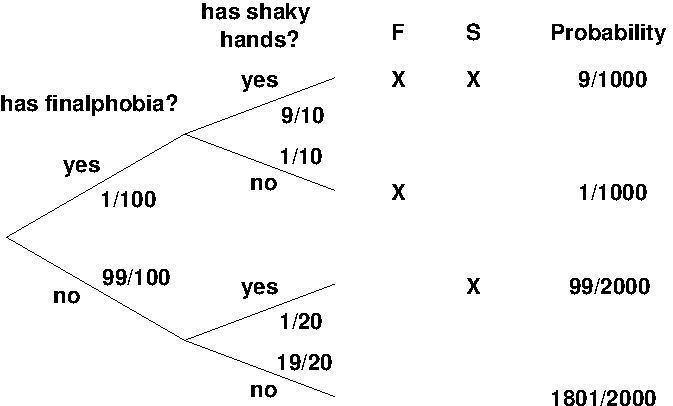
\includegraphics{finalphobia}
%\end{center}
%%
%The probability that a person has finalphobia, given that he or she
%has shaky hands is:
%%
%\begin{align*}
%\prcond{F}{S}
%    & = \frac{\pr{F \cap S}}{\pr{S}} \\
%        & = \frac{9/1000}{9/1000 + 99/2000} \\
%	    & = \frac{18}{18+99} \\
%	        & = \frac{18}{117}
%\end{align*}
%
%So, while it's true that someone with shaky hands is five times more likely to have finalphobia than someone with steady hands, it remains a poor bet---about 1 in 5---that someone with shaky hands actually has does have finalphobia.}
%
%\end{problem}


%%%%%%%%%%%%%%%%%%%%%%%%%%%%%%%%%
%%% Fall05 ps9 problem 1

\begin{problem}{20}
Professor Plum, Mr. Green, and Miss Scarlet are all plotting to shoot
Colonel Mustard.  If one of these three has both an
\textit{opportunity} and the \textit{revolver}, then that person shoots
Colonel Mustard.  Otherwise, Colonel Mustard escapes.  Exactly one of
the three has an \textit{opportunity} with the following
probabilities:
%
\begin{align*}
\pr{\text{Plum has opportunity}} & = 1 / 6 \\
\pr{\text{Green has opportunity}} & = 2 / 6 \\
\pr{\text{Scarlet has opportunity}} & = 3 / 6
\end{align*}
%
Exactly one has the \textit{revolver} with the following
probabilities, regardless of who has an opportuntity:
%
\begin{align*}
\pr{\text{Plum has revolver}} & = 4 / 8 \\
\pr{\text{Green has revolver}} & = 3 / 8 \\
\pr{\text{Scarlet has revolver}} & = 1 / 8
\end{align*}

\bparts

\ppart{5} Draw a tree diagram for this problem.  Indicate edge and
outcome probabilities.

\solution{
\begin{center}
\begin{picture}(120,270)(0,-30)
\put(0,120){\line(2,3){60}}
\put(0,120){\line(1,0){60}}
\put(0,120){\line(2,-3){60}}
\put(60,30){\line(2,-1){60}}
\put(60,30){\line(1,0){60}}
\put(60,30){\line(2,1){60}}
\put(60,120){\line(2,-1){60}}
\put(60,120){\line(1,0){60}}
\put(60,120){\line(2,1){60}}
\put(60,210){\line(2,-1){60}}
\put(60,210){\line(1,0){60}}
\put(60,210){\line(2,1){60}}
\put(30,180){\makebox(0,0){P}}
\put(30,130){\makebox(0,0){G}}
\put(30,60){\makebox(0,0){S}}
\put(110,245){\makebox(0,0){P}}
\put(110,220){\makebox(0,0){G}}
\put(110,175){\makebox(0,0){S}}
\put(110,155){\makebox(0,0){P}}
\put(110,130){\makebox(0,0){G}}
\put(110,85){\makebox(0,0){S}}
\put(110,65){\makebox(0,0){P}}
\put(110,40){\makebox(0,0){G}}
\put(110,-5){\makebox(0,0){S}}
\put(45,160){\makebox(0,0){$1/6$}}
\put(30,110){\makebox(0,0){$2/6$}}
\put(45,80){\makebox(0,0){$3/6$}}
\put(85,235){\makebox(0,0){$4/8$}}
\put(110,200){\makebox(0,0){$3/8$}}
\put(85,185){\makebox(0,0){$1/8$}}
\put(85,145){\makebox(0,0){$4/8$}}
\put(110,110){\makebox(0,0){$3/8$}}
\put(85,95){\makebox(0,0){$1/8$}}
\put(85,55){\makebox(0,0){$4/8$}}
\put(110,20){\makebox(0,0){$3/8$}}
\put(85,5){\makebox(0,0){$1/8$}}
\put(30,15){\makebox(0,0){\text{opportunity}}}
\put(90,-20){\makebox(0,0){\text{revolver}}}
\put(150,-20){\makebox(0,0){\text{prob.}}}
\put(150,240){\makebox(0,0){$4/48$}}
\put(150,210){\makebox(0,0){$3/48$}}
\put(150,180){\makebox(0,0){$1/48$}}
\put(150,150){\makebox(0,0){$8/48$}}
\put(150,120){\makebox(0,0){$6/48$}}
\put(150,90){\makebox(0,0){$2/48$}}
\put(150,60){\makebox(0,0){$12/48$}}
\put(150,30){\makebox(0,0){$9/48$}}
\put(150,0){\makebox(0,0){$3/48$}}
\end{picture}
\end{center}
}

\ppart{5} What is the probability that Colonel Mustard is shot?

\solution{Denote each outcome with a pair indicating who has the
opportunity and who has the revolver.  In this notation, the event
that Colonel Mustard is shot consists of all outcomes where a single
person has both:
%
\[
\set{(P,P),(G,G),(S,S)}
\]
%
The probability of this event is the sum of the outcome probabilities:
%
\begin{align*}
\pr{\set{(P,P),(G,G),(S,S)}}
    & = \pr{(P,P)} + \pr{(G,G)} + \pr{(S,S)} \\
    & = 4/48 + 6/48 + 3/48 \\
    & = 13/48
\end{align*}
}

\ppart{5} What is the probability that Colonel Mustard is shot, given
that Miss Scarlet does not have the revolver?

\solution{Let $S$ be the event that Colonel Mustard is shot, and let
$N$ be the event that Miss Scarlet does \textit{not} have the
revolver.  The solution is:
%
\begin{align*}
\prcond{S}{N}
    & = \frac{\pr{S \cap N}}{\pr{N}} \\
    & = \frac{\pr{(P,P),(G,G)}}{\pr{(P,P),(P,G),(G,P),(G,G),(S,P),(S,G)}} \\
    & = \frac{\frac{4}{48}+\frac{6}{48}}
             {\frac{4}{48}+\frac{3}{48}+\frac{8}{48}+
              \frac{6}{48}+\frac{12}{48}+\frac{9}{48}} \\
    & = \frac{5}{21}
\end{align*}
}

\ppart{5} What is the probability that Mr. Green had an opportunity,
given that Colonel Mustard was shot?

\solution{Let $G$ be the event that Mr. Green has an opportunity, and
again let $S$ be the event that Colonel Mustard is shot.  Then the
solution is:
%
\begin{align*}
\prcond{G}{S}
    & = \frac{\pr{G \cap S}}{\pr{S}} \\
    & = \frac{\pr{(G,G)}}{\pr{(P,P),(G,G),(S,S)}} \\
    & = \frac{\frac{6}{48}}
             {\frac{4}{48}+\frac{6}{48}+\frac{3}{48}} \\
    & = \frac{6}{13}
\end{align*}
}

\eparts

\end{problem}

%%%%%%%%%%%%%%%%%%%%%%%%%%%%%%%%%%%%%%%%%%%%%%%%%%%%%%%%%

%%%%%%%%%%%%%%%%%%%%%%%%%
%% fall 08, pset11

\begin{problem}{15}
In lecture we discussed the Birthday Paradox. Namely, we found that in a group of $m$ people with $N$ possible birthdays, if $m \ll N$, then:
\[
\pr{\text{all $m$ birthdays are different}} \sim e^{-\frac{m(m-1)}{2N}}
\]
To find the number of people, $m$, necessary for a half chance of a match, we set the probability to $1/2$ to get:
\[
m \sim \sqrt{(2\ln2)N} \approx 1.18\sqrt{N}
\]

For $N = 365$ days we found $m$ to be 23.

We could also run a different experiment. As we put on the board the birthdays of the poeple surveyed, we could ask the class if anyone has the same birthday. In this case, before we reached a match amongst the surveyed people, we would already have found other people in the rest of the class who have the same birthday as someone already surveyed. Let's investigate why this is.

\bparts
\ppart{5} Consider a group of $m$ people with $N$ possible birthdays amongst a larger class of $k$ people, such that $m \leq k$. Define $\pr{A}$ to be the probability that $m$ people all have different birthdays \textit{and} none of the other $k-m$ people have the same birthday as one of the $m$.

Show that, if $m \ll N$, then $\pr{A} \sim e^{\frac{m(m-2k)}{2N}}$. (Notice that the probability of no match is $e^{-\frac{m^2}{2N}}$ when $k$ is $m$, and it gets smaller as $k$ gets larger.)

\hspace{0.5in} \textit{Hints:} For $m \ll N$: $\frac{N!}{(N-m)!N^m} \sim e^{-\frac{m^2}{2N}}$, and $(1-\frac{m}{N}) \sim e^{-\frac{m}{N}}$.

\solution{
We know:
\[
\pr{A} = \frac{N(N-1)\ldots(N-m+1)\cdot(N-m)^{k-m}}{N^k}
\]

since there are $N$ choices for the first birthday, $N-1$ choices for the second birthday, etc., for the first $m$ birthdays, and $N-m$ choices for each of the remaining $k-m$ birthdays. There are total $N^k$ possible combinations of birthdays within the class.

\begin{align*}
\pr{A} &= \frac{N(N-1)\ldots(N-m+1)\cdot(N-m)^{k-m}}{N^k} \\
&= \frac{N!}{(N-m)!}\left(\frac{(N-m)^{k-m}}{N^k}\right) \\
&= \frac{N!}{(N-m)!N^m}\left(\frac{N-m}{N}\right)^{k-m} \\
&= \frac{N!}{(N-m)!N^m}\left(1-\frac{m}{N}\right)^{k-m} \\
&\sim e^{-\frac{m^2}{2N}} \cdot e^{-\frac{m}{N}(k-m)} & \text{(by the Hint)} \\
& = e^{\frac{m(m-2k)}{2N}}
\end{align*}
}

\ppart{10} Find the approximate number of people in the group, $m$, necessary for a half chance of a match (your answer will be in the form of a quadratic). Then simplify your answer to show that, as $k$ gets large  (such that $\sqrt{N} \ll k$), then $m \sim \frac{N\ln2}{k}$.

\hspace{0.5in} \textit{Hint:} For $x \ll 1$: $\sqrt{1-x} \sim (1-\frac{x}{2})$.

\solution{
Setting $\pr{A} = 1/2$, we get a solution for $m$:

\begin{align*}
1/2 &= e^{\frac{m(m-2k)}{2N}} \\
-2N\ln2 &= m^2 -2km  \\
0 &= m^2-2km + (2N\ln2) \\
m &= \frac{2k \pm \sqrt{(2k)^2 - 4(2N\ln2)}}{2}
\end{align*}

Simplifying the solution under the assumption of large $k$, we find:
\begin{align*}
m &= \frac{2k - \sqrt{4k^2 - 8N\ln2}}{2} & \text{(taking the lower positive root)} \\
&= k - k\sqrt{1 - \frac{2N\ln2}{k^2}} \\
&\sim k  - k \left(1-\frac{2N\ln2}{2k^2}\right) & \text{(by the Hint)} \\
&= \frac{N\ln2}{k}  
\end{align*}
}

\eparts

\end{problem}

%%%%%%%%%%%%%%%%%%%%%%%%%
%% fall 08, pset11

\instatements{\vspace{0.5in}}
\begin{problem}{10}
We're covering probability in 6.042 lecture one day, and you volunteer for one of Professor Leighton's demonstrations. He shows you a coin and says he'll bet you \$1 that the coin will come up heads. Now, you've been to lecture before and therefore suspect the coin is biased, such that the probability of a flip coming up heads, $\pr{H}$, is $p$ for $1/2 < p \leq 1$.

You call him out on this, and Professor Leighton offers you a deal. He'll allow you to come up with an algorithm using the biased coin to \textit{simulate} a fair coin, such that the probability you win and he loses, $\pr{W}$, is equal to the probability that he wins and you lose, $\pr{L}$. You come up with the following algorithm:

\begin{enumerate}
\item Flip the coin twice.
\item Based on the results:
	\begin{itemize}
	\item $TH \implies$ you win [$W$], and the game terminates.
	\item $HT \implies$ Professor Leighton wins [$L$], and the game terminates.
	\item $(HH \lor TT) \implies$ discard the result and flip again.
	\end{itemize}
\item If at the end of $N$ rounds nobody has won, declare a tie.
\end{enumerate}
As an example, for $N=3$, an outcome of $HT$ would mean the game ends early and you lose, $HHTH$ would mean the game ends early and you win, and $HHTTTT$ would mean you play the full $N$ rounds and result in a tie.

\bparts

\ppart{5}
Assume the flips are mutually independent. Show that $\pr{W} = \pr{L}$.

\solution{
The probability of you winning is equal to the probability that you win in the first round, plus the probability that nobody won in the first round times the probability that you win in the second round, plus the probability that nobody won in the first two round times the probability that you win in the third round, etc. The same goes for Professor Leighton. Hence:
\begin{align*}
\pr{W} &= \pr{TH} + \pr{HH \lor TT}\pr{TH} + \pr{HH \lor TT}^2\pr{TH} + \ldots \\
& = \pr{TH} \cdot \sum_{i=0}^N \pr{HH \lor TT}^i \\
& = \pr{HT} \cdot \sum_{i=0}^N \pr{HH \lor TT}^i\\
& = \pr{L}
\end{align*}
The middle step is possible because $\pr{TH} = (1-p)p = p(1-p) = \pr{HT}$.
}

\ppart{5}
Show that, if $p<1$, the probability of a tie goes to 0 as $N$ goes to infinity.

\solution{
The probability of a tie is just the probability that nobody won all $N$ rounds, namely:
\[
\pr{tie} = (\pr{HH \lor TT})^N = (\pr{HH} + \pr{TT})^N = (p^2 + (1-p)^2)^N
\]
So the limit as $N$ goes to infinity is 0, given that $p$ and therefore $p^2 + (1-p)^2$ are $< 1$.
}

\eparts

\end{problem}

%%%%%%%%%%%%%%%%%%%%%%%%%
%% Spring08, Pset 11, Problem 7
\begin{problem}{20}

\bparts

\ppart{5} Suppose $A$ and $B$ are \emph{disjoint} events.  Prove that $A$ and
$B$ are \emph{not independent}, unless $\prob{A}$ or $\prob{B}$ is zero.

\solution{ Since $A$ and $B$ are disjoint, 
\[
\prob{A \intersect B} =  \prob{\emptyset}  = 0.
\]
So, $\prob{A \intersect B}=\prob{A} \cdot \prob{B}$ iff $\prob{A}=0$ or $\prob{B}=0$.
}


\ppart{5} If $A$ and $B$ are independent, prove that $A$ and $\bar{B}$
are also independent.

\textit{Hint:  $\prob{A \intersect \bar{B}} = \prob{A} - \prob{A \intersect B}$.}

\iffalse

You may find it useful to use results from Problem
\ref{Identities}.

Problem \ref{Identities} (\ref{setminus})
\fi

\solution{
\begin{align*}
\prob{A \intersect \bar{B}}
% &= \prob{A - B} \\
 &= \prob{A} - \prob{A \intersect B} &&\text{(by the hint)} \\
 &= \prob{A} - \prob{A} \cdot \prob{B} &&\text{(since $A$ and $B$ are independent)} \\
 &= \prob{A} \cdot (1 - \prob{B}) \\
 &= \prob{A} \cdot \prob{\bar{B}}.
\end{align*}
The last equality holds since the probability of any event equals $1$ minus the probability of its
complement.
Thus, we have shown that $\prob{A \intersect \bar{B}}=\prob{A} \cdot \prob{\bar{B}}$,
which is equivalent to $A$ and $\bar{B}$ being independent.
}


\ppart{5} 
Give an example of events $A$,$B$, $C$ such that $A$ is independent of $B$,
$A$ is independent of $C$, but $A$ is not independent of $B\union C$.

\solution{The experiment is 2 independent coin flips, letting $A$ be ``the
1st flip is heads'', $B$ the ``the 2nd flip is heads,'' $C$ is ``odd
number of heads.''  Then $A$ is not independent of $B \union C$ because
\[
\prcond{A}{B \union C}= \frac{\prob{A \intersect (B \union C)}}{\prob{B \union C}}= \frac{\prob{HH,HT}}{\prob{HH,TH,HT}} = 2/3 \neq 1/2 = \prob{A}.
\]

\iffalse

Consider the usual random experiment of
rolling a die and let $A$, $B$, $C$ be the events that the die rolls
less than 3, rolls an even number, or rolls a prime number,
respectively. I.e., 
\[
A = \{1,2\} \qquad
B = \{2,4,6\} \qquad
C = \{2,3,5\}.
\]
Then, 
$$
\prob{A}=\tfrac{1}{3}, 
\qquad
\prob{B}=\prob{C}=\tfrac{1}{2},
$$
and
$$
\prob{A\cap B}=
\prob{A\cap C}=
\prob{B\cap C}=
\prob{A\cap B\cap C}=
\prob{\{2\}}=
\tfrac{1}{6}.
$$
Easily, 
$$
\prob{A\mid B}=
\prob{A\mid C}=
\tfrac{1}{6}/\tfrac{1}{2}=
\tfrac{1}{3}=
\prob{A},
$$
which proves $A$ is independent of $B$ and also independent of
$C$. However, 
$$
\prob{A\mid B\cap C}=
\prob{A\cap B\cap C}/\prob{B\cap C}=
\tfrac{1}{6}/\tfrac{1}{6}=
1\neq
\prob{A},
$$
which implies $A$ is not independent of $B\cap C$.
\fi

}

\ppart{5} Prove that if $C$ is independent of $A$, and $C$ is independent of
$B$, and $C$ is independent of $A \intersect B$, then $C$ is independent
of $A \union B$.

\textit{Hint:} Calculate $\prcond{A \union B}{C}$.

\solution{
Conditional inclusion-exclusion followed by plain inclusion-exclusion provides
a quick proof:
\begin{align*}
\prcond{A \union B}{C}
 &= \prcond{A}{C} + \prcond{B}{C} - \prcond{A \intersect B}{C}
    & \text{(by conditional inc-ex)}\\
 &= \prob{A} + \prob{B} - \prob{A \intersect B}
    &\text{(by independence)} \\
 &= \prob{A \union B}
    & \text{(by regular inc-ex)}
\end{align*}
}
\eparts
\end{problem}

%%%%%%%%%%%%%%%%%%%%%%%%%%%%%%%%%%%%%%%%%%%%%%%%%%%%%%%%%%
%New problem
\begin{problem}{15}
Three very rare DNA markers were found in the DNA collected at a crime scene. Only one in every $1,000$ people has marker $A$, one in every $3,000$ people has marker $B$, and one in every $5,000$ people has marker $C$. Joe the plumber was arrested and accused of committing the crime, because he had all those markers present in his DNA. The prosecutor argues that the chances of any person having all three DNA markers is \[\frac1{1000}\cdot\frac{1}{3000}\cdot \frac1{5000} = \frac{1}{15,000,000,000}\], which is more than $1$ over the number of people in the world. This, plus the fact that Joe the plumber lives only 100 miles away from the crime scene must clearly mean that he is guilty. Having taken $6.042$, you should be suspicious of this reasoning.
\bparts
\ppart{2}
What assumption has the prosecutor made (even though he hasn't realized it) about the presence of the $3$ markers in human DNA?
\solution{Mutual independence.}
\ppart{4}
What would be the probability of a person having all three markers assuming that the markers appear pairwise independently? Under this assumption, can it be stated with such certainty that Joe the plumber commited the crime?
\solution{\[Pr[A\intersect B \intersect C] \leq Pr[B \intersect C] = Pr[B]\cdot Pr[C] = \frac{1}{15,000,000}\]
One in $15,000,000$ people might have all the three markers, and the fact that Joe the plumber lives $100$ miles away means nothing if the crime was committed in, say, New York City.}
\ppart{4}
What can you say about the probability of a person having all three markers if there is no independence between the markers?
\solution{The probability is at most \[P[C] = \frac{1}{5,000}.\]}
\ppart{5}
In fact, it turns out that neither of the above assumptions is correct. A researcher from MIT (who was actually in your recitation section for 6.042 back in the day) has discovered that while markers B and C appear independently, the probability of having marker B if you have marker A is $\frac12$ and the probability of having marker C if you have marker A is $\frac13$. The defence attorney now argues that the probability of a randomly selected person having all three markers is 
\[Pr[A\intersect B\intersect C] = Pr[A]\cdot Pr[B|A] \cdot Pr[C|A] =  \frac{1}{1000} \cdot \frac12 \cdot \frac13 = \frac{1}{6,000}.\]
Called as a witness, the MIT researcher points out that this is not necessarily true and that in fact he himself does not know what the probability is. What is wrong with the defence attorney's reasoning? (We assume that the MIT researcher published correct information and that, since he took 6.042, he knows what he is talking about.)
\solution{The researcher said that markers B and C appear independently, but he never said that they are independent if the person has marker A.}
\eparts
\end{problem}

\end{document}